\iflanguage{ngerman}
{\chapter{Ergebnisse}}
{\chapter{Results}}

\label{sec:results}


% Linerenderer conponent also produces large overhead due to the amount of gameobjects it creates
% Need to test when Dataset gets to large for my PC to handle
% Also add expert feedback
% objektive comparison of presented methods 
% Forced based approach spacing force F_s needs imporvment as algorithm is slow (O(n^2))
% informal quality analysis? 
% waht could be done to improve the visuallisation of dynamic datasetss?
% Are exploded Views really viable for that?
This chapter illustrates the implemented methods.
The visualization of the data set can be seen in Figure \ref{fig:PointExplosionPicture}. Here the point explosion was used to explode the cell.
The dataset contains three different cell populations, which are colored orange, green and blue. The colors are set randomly at the start of the program when a new population is found in the dataset. Orange is the cell population named "cells", the population "cells\_inner" is green, and the "lumen" is the largest blue colored cell around the center.
Also small green dots can be seen in the cell center. These mark the initial center of mass of the cell, which is used as the reference point to create the exploded view.
\begin{figure}[h]
	\centering
	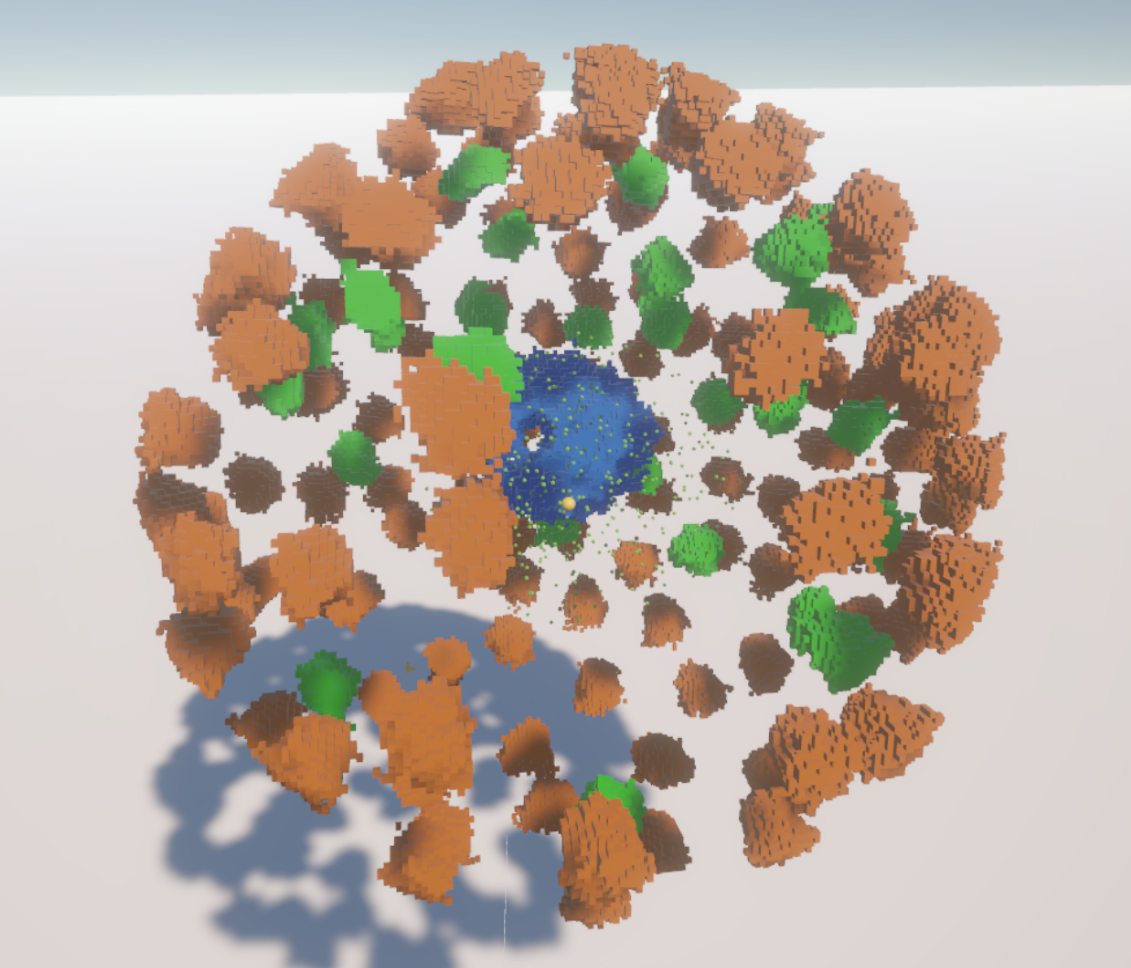
\includegraphics[width=.6\linewidth]{fig/Images/PointExplosionPicture}
	\caption[]{Point explosion of the dataset. The different cell populations were marked in orange, green and blue. }
	\label{fig:PointExplosionPicture}
\end{figure}

Figure \ref{fig:LineExplosionPictures} shows the data set as it is transformed with the line explosion. The yellow arrow indicates the axis on which the parts are projected as described in chapter \ref{lineExp}. 
The yellow arrow is an interactable and can be positioned by the user. 
The three pictures show different parameter combinations of the factors $F=(F_1, F_2, F_3)$. So here on the left picture each part is translated along the line without influencing the distance of the parts to the axis.  
This can be achieved with $F=(1,0,0)$ and allows the expansion along the axis, similar to drawn explosion views. The object structure remains largely intact and is merely pulled apart. It can also be seen that the control point $P_s$ was placed inside the cell complex, and thus only the right half of the data set is expanded. 
\begin{figure}[t]
	%\centering
	%\noindent
	%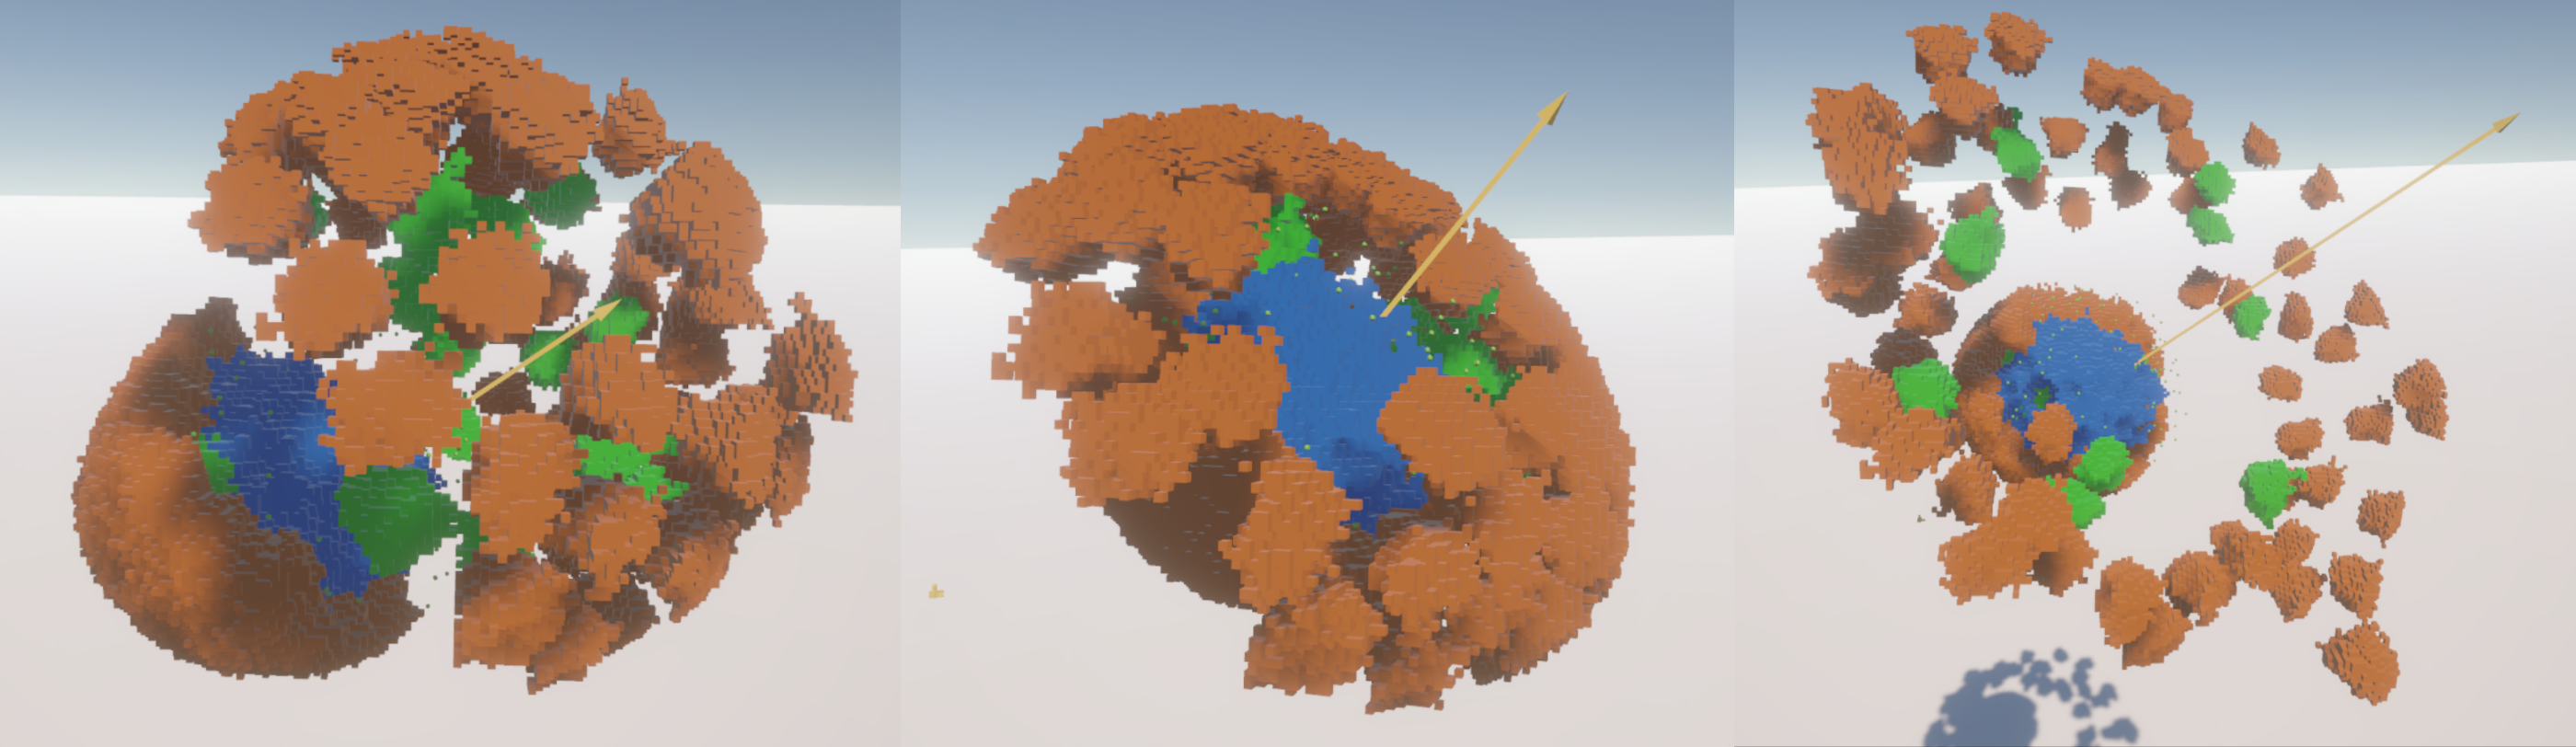
\includegraphics[width=1\paperwidth]{fig/Images/LineExplosionPictures}
	\noindent\makebox[\textwidth]{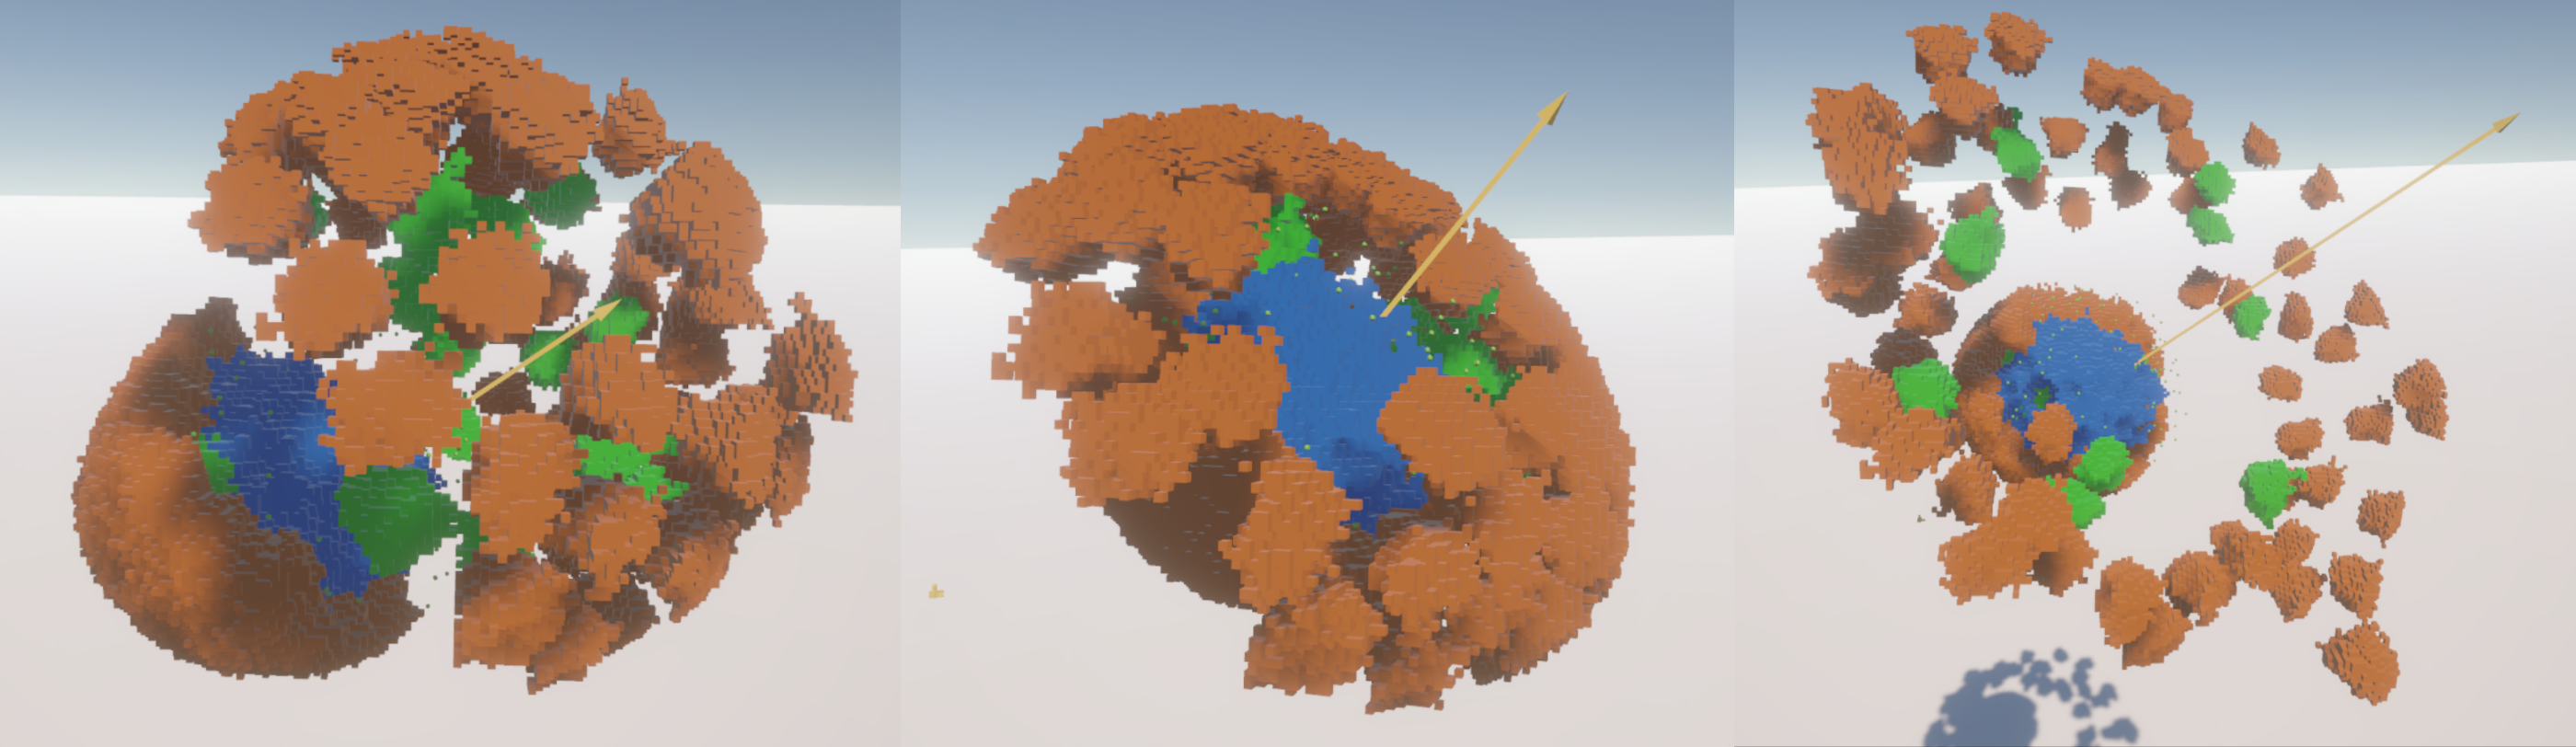
\includegraphics[width=1.025\paperwidth]{fig/Images/LineExplosionPictures}}
	\caption[]{Different lines explosions created with different factor combinations of the parameters $F=(F_1, F_2, F_3)$. On the left $F=(1,0,0)$, in the middle $F=(0, 0, 1)$ and on the right $F=(0.3, 1, 0)$.}
	\label{fig:LineExplosionPictures}
\end{figure}
In the middle picture you can see the factor combination $F=(0, 0, 1)$, which pushes the parts from their original position outwards, away from the line. 
This allows a clear view of the inside of the object. 
Interesting is the factor combination $F=(0.3, 1, 0)$, which can be seen in the right picture of Figure \ref{fig:LineExplosionPictures}. Here a conical explosion is created which shows the inside of the object and also allows a clear view of the individual parts.  
Since the parameters can be adjusted via the UI panel at runtime, an analytical inspection is possible, as the best view can easily be found by adjusting the factors as needed.   
Figure \ref{fig:HeadMountedLineExplosion} shows the extension of the line explosion to be view-dependent. Here, the point $P_s$ was also placed inside the cell complex, pushing all occluding parts out of the view of the observer. 
On the right graphic, the lumen, i.e. the blue cell, was taken by the user, thus allowing an unobstructed view of the cells behind it or on the lumen itself.  
\begin{figure}[h]
	\centering
	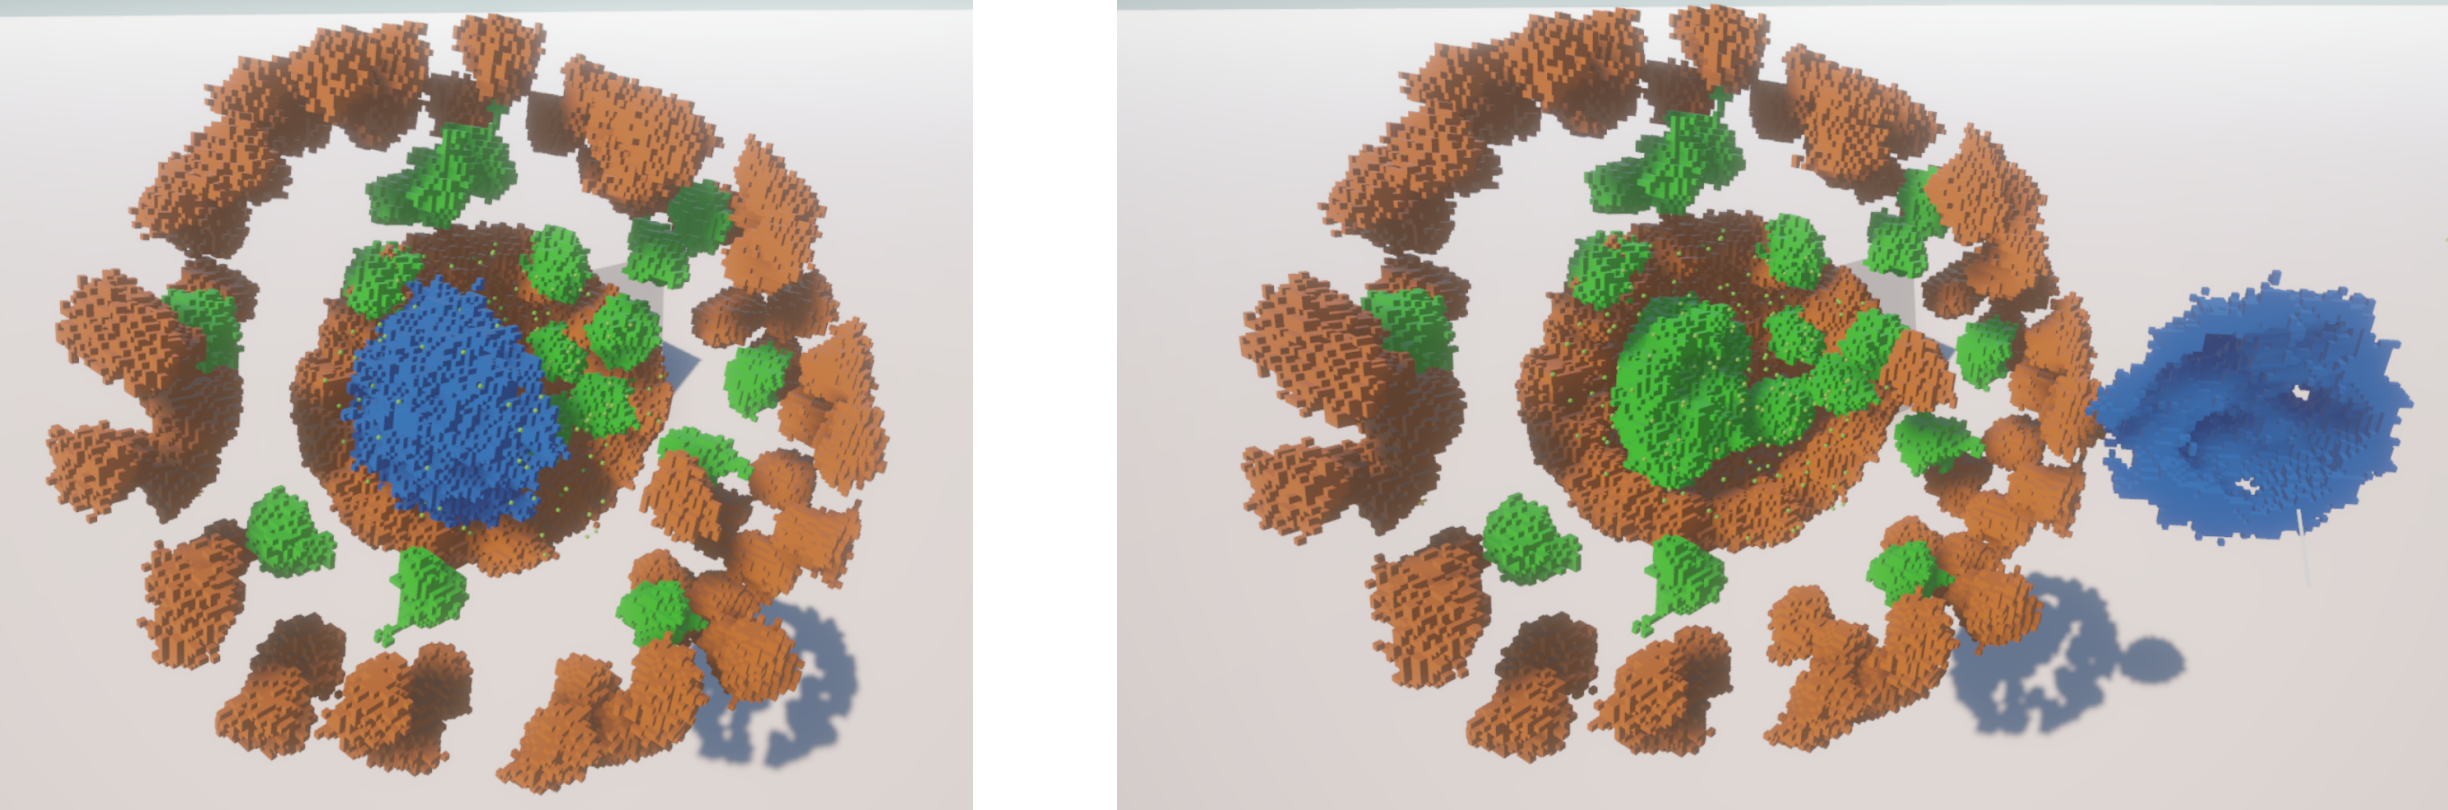
\includegraphics[width=1\linewidth]{fig/Images/HeadMountedLineExplosion}
	\caption[]{Extension of the line explosion to produce a view-dependent representation. On the right, the lumen, i.e. the blue cell, was taken out by the user to allow a clear view on the cells behind it.  }
	\label{fig:HeadMountedLineExplosion}
\end{figure}

Figure \ref{fig:ForceBasedExplosionPicture} shows the force-based explosion. Here, three cells were selected from which the explosion originates. These selected parts remain in their original position, while all other parts are pushed away.
In the left of the two images, the viewingforce has been increased so that all parts that are not selected are pushed out of the line of sight and the target parts can be seen clearly.     
On the right image, the viewingforce has been set to zero, which means that all parts are pushed away, but the object structure is broken up less.
\begin{figure}[t]
	\centering
	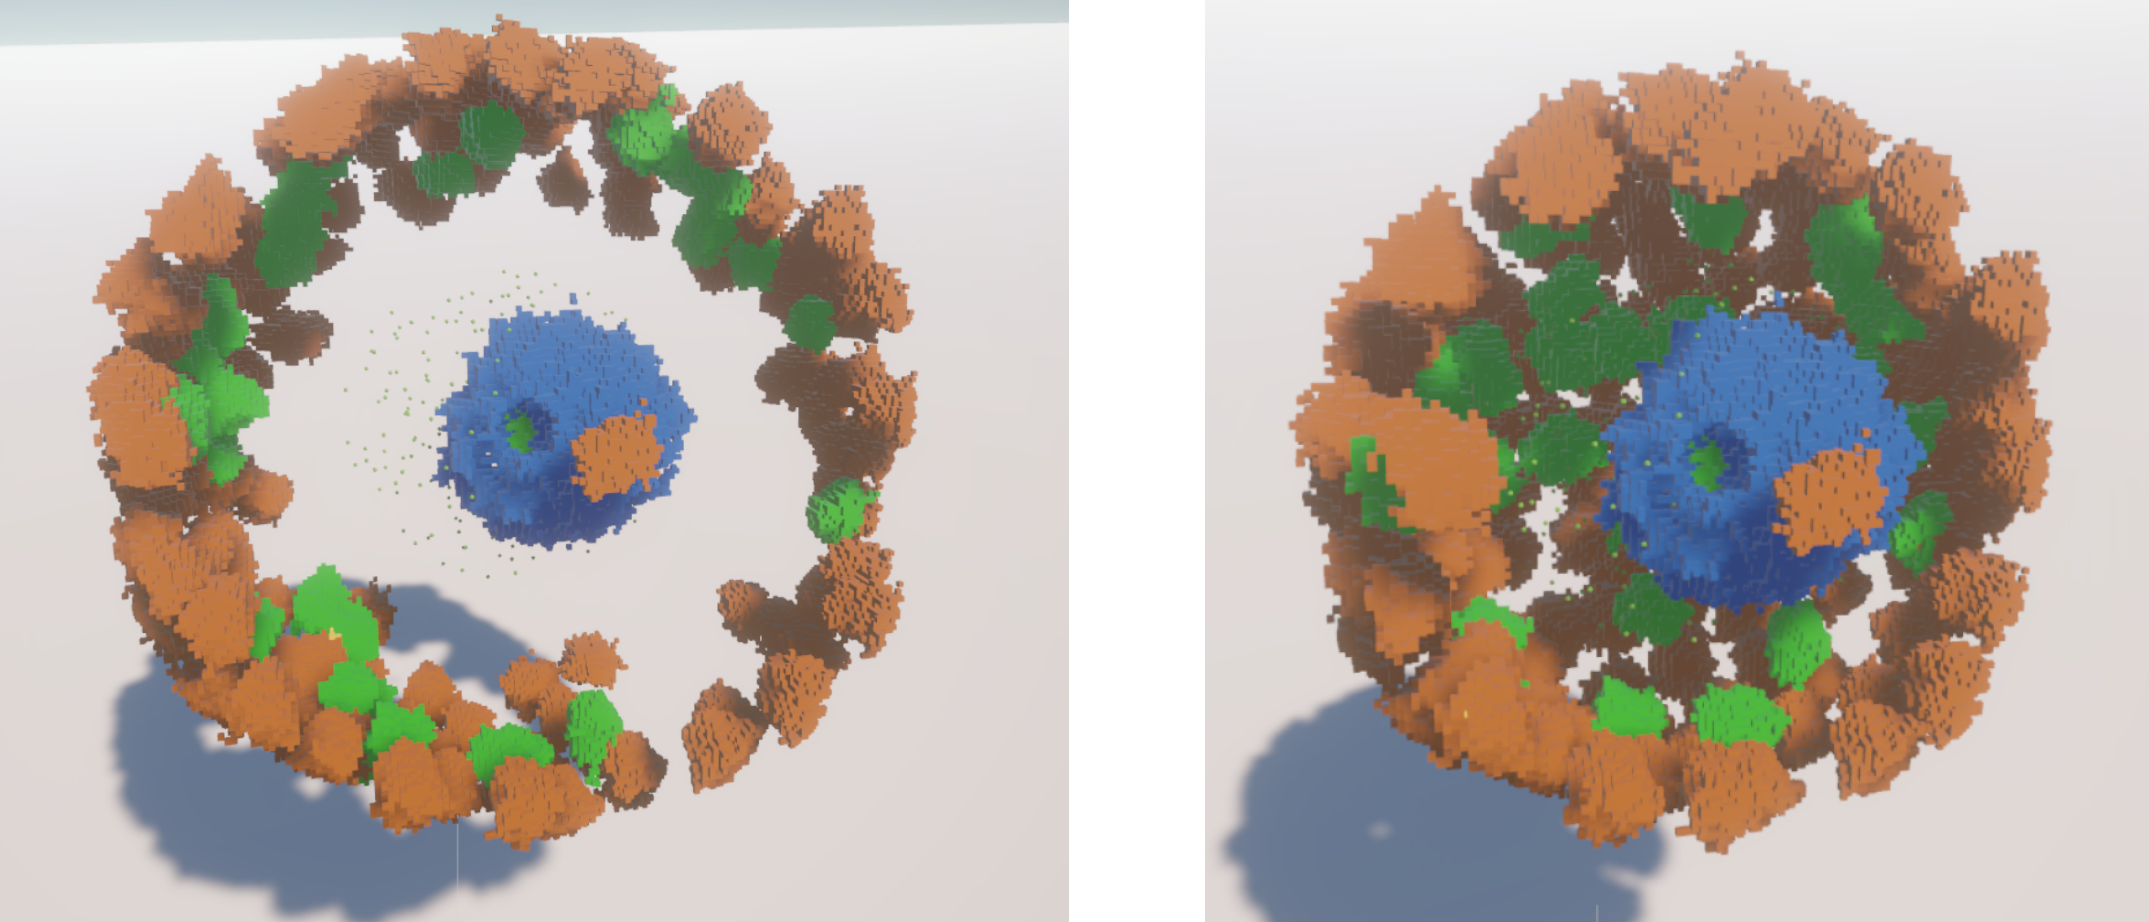
\includegraphics[width=1\linewidth]{fig/Images/ForceBasedExplosionPicture}
	\caption[]{Force-based explosion, left with viewingforce, on the right the viewingforce is set to zero. }
	\label{fig:ForceBasedExplosionPicture}
\end{figure}
Figure \ref{fig:TransparencyAndUI} shows the UI panel with which the user can interact and adjust the parameters of the explosion views. Furthermore, the time control can be seen on the left. On the right side the population and ID of the selected cell is displayed.  
Also, a cell was taken and held in front of the panel to show the transparency, which shows the change of the cell since the last time step. This can also be seen in figure \ref{fig:ChangeOfCellTranparent} in the appendix, with the lumen cell of another simulation. 
\begin{figure}[h]
	\centering
	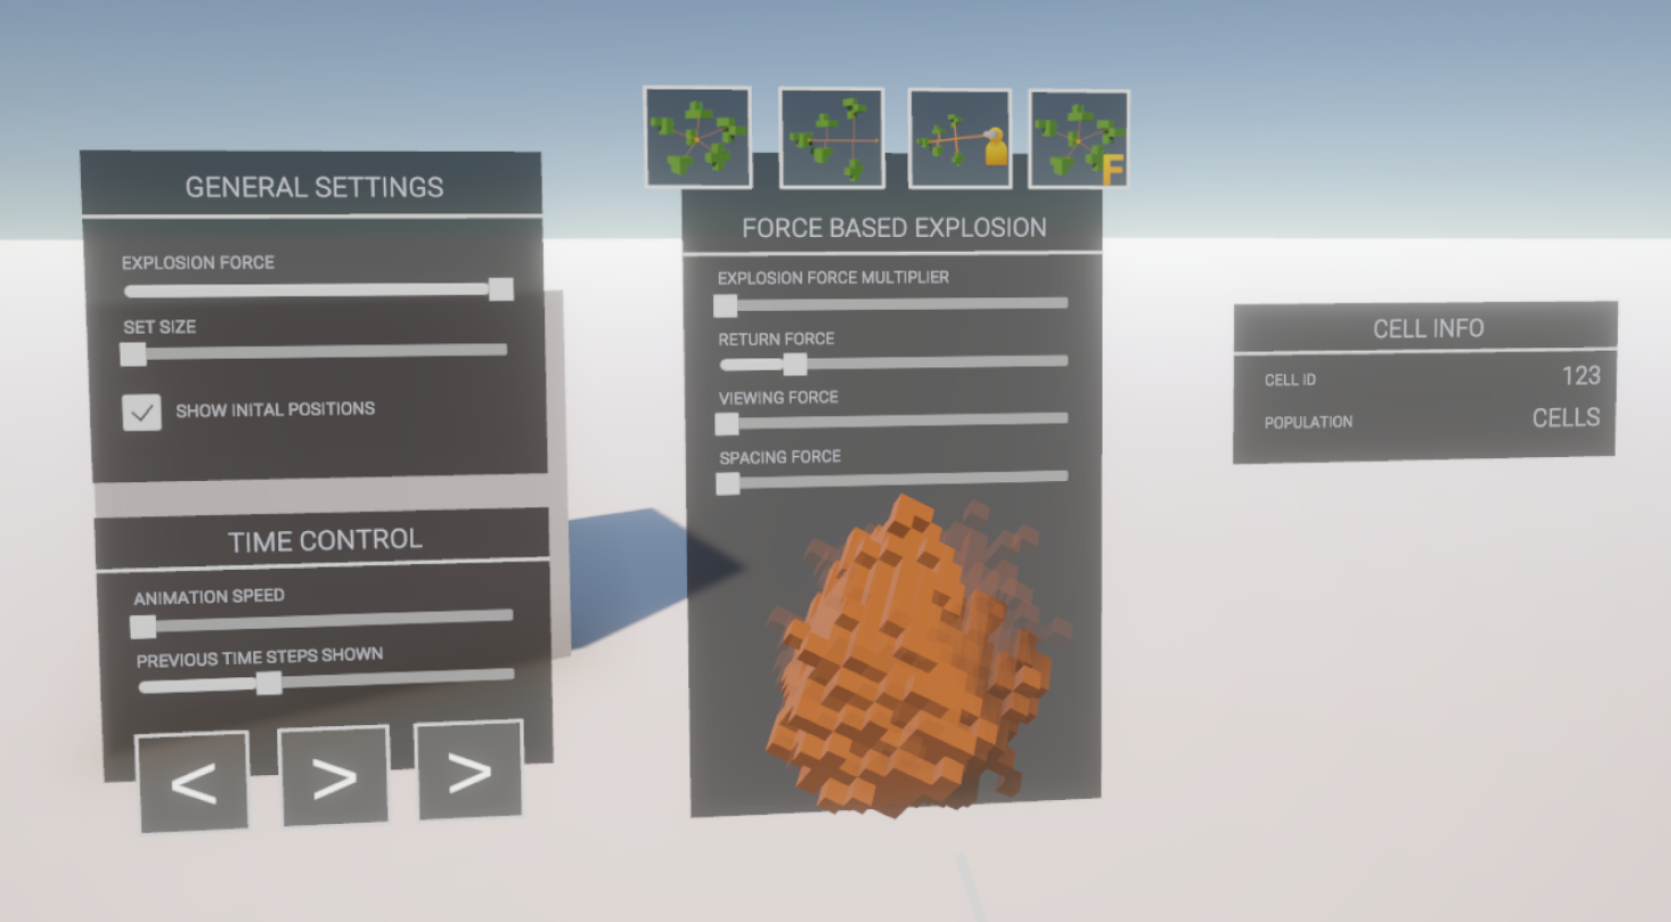
\includegraphics[width=1\linewidth]{fig/Images/TransparencyAndUI}
	\caption[]{UI panel with which the user can adjust the parameters of the explosion and the time. A cell is held in front of the panel to show the transparency, which visualizes the change of the cell with respect to the last time step. }
	\label{fig:TransparencyAndUI}
\end{figure}













